\documentclass[11pt]{article}

\usepackage{a4wide}
\usepackage[utf8]{inputenc}
\usepackage[russian]{babel}
\usepackage{graphicx}
\usepackage{amsmath}
\usepackage{amsthm}
\usepackage{amssymb}

\newtheorem{theorem}{Теорема}
\newtheorem{definition}{Определение}
\newtheorem{proposition}{Утверждение}

\newcommand*{\hm}[1]{#1\nobreak\discretionary{}{\hbox{$\mathsurround=0pt #1$}}{}}
\newcommand\abs[1]{\left\lvert#1\right\rvert}
\newcommand{\scalar}[2]{\left<#1,#2\right>}
\newcommand{\norm}[1]{\left\lVert #1 \right\lVert}
\renewcommand{\d}[1]{\ensuremath{\operatorname{d}\!{#1}}}

\begin{document}
\thispagestyle{empty}

\begin{center}
\ \vspace{-3cm} \newline
\includegraphics[width=0.5\textwidth]{msu.eps}\\
{\scshape Московский государственный университет имени М.~В.~Ломоносова}\\
Факультет вычислительной математики и кибернетики\\
Кафедра системного анализа

\vfill

{\LARGE Курсовая работа} \newline
%\vspace{1cm}
{\Huge\bfseries Изучение динамических систем с дискретным временем}
\end{center}

\vspace{1cm}
\begin{flushright}
\large
\textit{Студент 315 группы}\\
В.~С.~Терёшин\\
\vspace{5mm}
\textit{Преподаватель}\\
д.ф.-м.н., профессор А.~С.~Братусь
\end{flushright}

\vfill
\begin{center}
Москва, 2014
\end{center}
\pagebreak
\tableofcontents
\pagebreak
\section{Постановка задачи}
Дана дискретная динамическая система, описывающая некую модель популяции планктона:
\begin{gather}
u_{t+1} = u_t \exp\left\{\frac{0.081}{u_t} - \frac{0.001}{u_t^2} - 0.305\right\}, \notag \\
\left. u_t \right|_{t = 0} = u_0, \; \; \; u_0 > 0. \notag
\end{gather}
Необходимо для данной системы:
\begin{enumerate}
\item
Найти неподвижные точки отображения и исследовать их устойчивость;
\item
Исследовать систему на наличие циклов длины два;
\item
Исследовать систему на наличие циклов длины три;
%\item
%Построить бифуркационную диаграмму;
\item
Построить графики показателя Ляпунова.
\end{enumerate}

%Также дана вторая система, двумерная:
%$$
%n_{t+1} = n_t \exp{ \left\{ \frac{0.081}{n_t} - \frac{0.001}{n_{t-1}^2} - 0.305 \right\} }.
%$$
%Для неё необходимо
\section{Неподвижные точки отображения и их устойчивость}
\begin{definition}
Точка $u_*$ называется неподвижной, если $u^* = f(u^*)$.
\end{definition}
Очевидно, что точка $u_0^* = 0$ является неподвижной.

Найдём остальные неподвижные точки отображения:
$$
u \exp\left\{\frac{0.081}{u} - \frac{0.001}{u^2} - 0.305\right\} = u.
$$
Так как $u \neq 0$, то можно данное уравнение поделить на $u$:
$$
\exp\left\{\frac{0.081}{u} - \frac{0.001}{u^2} - 0.305\right\} = 1,
$$
что эквивалентно
\begin{gather}
\frac{0.081}{u} - \frac{0.001}{u^2} - 0.305 = 0 \notag \\
0.305 u^2 - 0.081 u + 0.001 = 0. \notag
\end{gather}
Откуда неподвижные точки равны:
$$
u_1^* = \frac{0.081 - \sqrt{0.005341}}{0.61} \approx 0.01298008924, \; \; \; u_2^* = \frac{0.081 + \sqrt{0.005341}}{0.61} \approx 0.25259368125.
$$
\subsection{Устойчивость}
\begin{definition}
Неподвижная точка $u^*$ устойчива, если для любого $\varepsilon > 0$ существует $\delta(\varepsilon) > 0$ такое, что $\abs{u_0 - u^*} < \delta$, то $\abs{u_t - u^*} < \varepsilon$ для любого натурального $t$.\\
Если $\lim\limits_{t \to \infty} u_t = u^*$, то точка $u^*$ называется ассимпотически устойчивой.
\end{definition}
\begin{proposition}[Достаточное условие устойчивости]
Пусть $u^*$ --- неподвижная точка и $\abs{f'\left(u^*\right)} < 1$. Тогда $u^*$ устойчива и ассимптотически устойчива. Если $\abs{f'\left(u^*\right)} > 1$, то точка $u^*$ не является устойчивой.
\end{proposition}
В данной системе
$$
f(u) = u \exp\left\{ \frac{0.081}{u} - \frac{0.001}{u^2} - 0.305 \right\},
$$
а производная равна
\begin{gather}
f'(u) = \exp\left\{ \frac{0.081}{u} - \frac{0.001}{u^2} - 0.305 \right\} + u \exp\left\{ \frac{0.081}{u} - \frac{0.001}{u^2} - 0.305 \right\} \left( -\frac{0.081}{u^2} + \frac{0.002}{u^3} \right) = \notag \\
= \exp\left\{ \frac{0.081}{u} - \frac{0.001}{u^2} - 0.305 \right\} \left( 1 + \frac{0.002}{u^2} - \frac{0.081}{u} \right). \notag
\end{gather}
\subsubsection{Точка $u_1^*$}
\begin{gather}
f'(u_1^*) = f'\left(\frac{0.081 - \sqrt{0.005341}}{0.61}\right) \approx 6.630326895276139 \notag \\
\abs{f'(u_1^*)} > 1, \notag
\end{gather}
а значит, неподвижная точка $u_1^*$ не является устойчивой, то есть является репеллером.
\subsubsection{Точка $u_2^*$}
\begin{gather}
f'(u_2^*) = f'\left(\frac{0.081 + \sqrt{0.005341}}{0.61}\right) \approx 0.710673104723859 \notag \\
\abs{f'(u_2^*)} < 1, \notag
\end{gather}
а значит, неподвижная точка $u_2^*$ является устойчивой, то есть является аттрактором.
\section{Циклы длины два}
\begin{definition}[Цикл длины $m$]
$f(u)$ имеет цикл длины $m$, если существуют $u_1, u_2, \ldots, u_m$ такие, что $u_2 = f(u_1), u_3 = f(u_2), \ldots, u_m = f(u_{m-1}), u_1 = f(u_m)$, но $u_i \neq u_j$ если $i \neq j$.
\end{definition}

Установим наличие или отсутствие в данной системе циклов длины два. Рассмотрим следующее изображение:

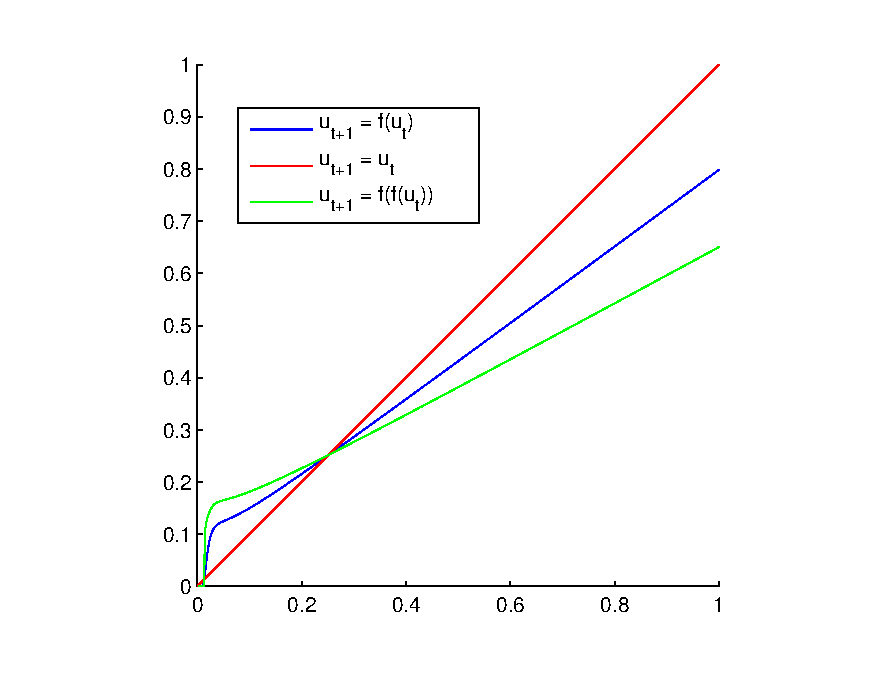
\includegraphics[scale=1.0]{pics/f_ff.eps}

Из графика видно, что $f(f(u)) < f(u) < u$ при $0 = u_0^* < u < u_1^*$ и при $u > u_2^*$, но $u < f(u) < f(f(u))$ при $u_1^* < u < u_2^*$. Докажем это формально.

Сначала докажем отношения между $u$ и $f(u)$ на указанных промежутках. Для этого необходимо оценить знак выражения:
$$
\frac{0.081}{u} - \frac{0.001}{u^2} - 0.305.
$$
Найдём, когда оно будет отрицательным:
\begin{gather}
\frac{0.081}{u} - \frac{0.001}{u^2} - 0.305 < 0, \notag \\
0.305 u^2 - 0.081 u + 0.001 > 0. \notag
\end{gather}
Откуда получим ответ на поставленный вопрос: выражение отрицательно при $0 = u_0^* < u < u_1^*$ и при $u > u_2^*$. Аналогично получим, что оно положительно при $u_1^* < u < u_2^*$.
Из этого следует, что опредено отношение между $\exp\left\{ \frac{0.081}{u} - \frac{0.001}{u^2} - 0.305 \right\}$ и $1$. А из этого получаем те же отношения между $f(u)$ и $u$, как было указано выше.

Оценим теперь отношение между $f(u)$ и $f(f(u))$ в указанных промежутках. Для этого оценим знак выражения:
\begin{gather}
\frac{0.081}{u \exp\left\{ \frac{0.081}{u} - \frac{0.001}{u^2} - 0.305 \right\}} - \frac{0.001}{u^2 \left(\exp\left\{ \frac{0.081}{u} - \frac{0.001}{u^2} - 0.305 \right\}\right)^2} - 0.305 = \notag \\
= \frac{0.081}{f(u)} - \frac{0.001}{\left( f(u) \right)^2} - 0.305. \notag
\end{gather}
Это выражение отрицательно, если $0 = u_0^* < f(u) < u_1^*$ или $f(u) > u_2^*$, и положительно, если $u_1^* < f(u) < u_2^*$.

Покажем, что $f(u)$ возрастает при положительных $u$. Для этого рассмотрим её производную:
$$
f'(u) = \exp\left\{ \frac{0.081}{u} - \frac{0.001}{u^2} - 0.305 \right\} \left( 1 + \frac{0.002}{u^2} - \frac{0.081}{u} \right).
$$
Её знак совпадает со знаком $1 + \tfrac{0.002}{u^2} - \tfrac{0.081}{u}$. Найдём, когда это выражение положительно:
\begin{gather}
1 + \tfrac{0.002}{u^2} - \tfrac{0.081}{u} > 0, \notag \\
u^2 - 0.081 u + 0.002 > 0. \notag
\end{gather}
Данный квадратный трёхчлен не имеет корней, следовательно, он положителен при всех значениях $u$. А значит, $f(u)$ возрастает при всех $u$. Следовательно, $0 = u_0^* < f(u) < u_1^*$ при $0 = u_0^* < u < u_1^*$ и $f(u) > u_2^*$ при $u > u_2^*$. Аналогично $u_1^* < f(u) < u_2^*$ при $u_1^* < u < u_2^*$.

Отсюда следует, что $f(f(u)) < f(u)$ при $0 = u_0^* < u < u_1^*$ и $u > u_2^*$ и $f(f(u)) > f(u)$ при $u_1^* < u < u_2^*$. А значит, $f(f(u)) < f(u) < u$ при $0 = u_0^* < u < u_1^*$ и при $u > u_2^*$, но $u < f(u) < f(f(u))$ при $u_1^* < u < u_2^*$.

Значит, не существует точек $u^{**} \geqslant 0$ таких, что $f(f(u^{**})) = u^{**}$, но $f(u^{**}) \neq u^{**}$. А значит, у данной системы не существует циклов длины два.
\section{Циклы длины три}
Вопрос о существовании циклов длины три решает следующая теорема. Упорядочим натуральные числа следующим образом:
$$
3 \rightarrow 5 \rightarrow 7 \rightarrow \ldots \rightarrow 3 \cdot 2 \rightarrow 5 \cdot 2 \rightarrow 7 \cdot 2 \rightarrow \ldots \rightarrow 3 \cdot 2^k \rightarrow 5 \cdot 2^k \rightarrow 7 \cdot 2^k \rightarrow \ldots \rightarrow 2^3 \rightarrow 2^2 \rightarrow 2 \rightarrow 1.
$$
\begin{theorem}[Шарковского]
Пусть дискретная динамическая система с непрерывным $f$ имеет цикл длины $n$. Тогда она имеет циклы длины $m$ для всех $m$ таких, что $n \rightarrow m$.
\end{theorem}

Из этой теоремы легко видеть, что в данной системе не существует циклов длины три. В противном случае существовали бы и циклы длины два, но в предыдущем параграфе было показано, что это не так.
\section{Показатели Ляпунова}
В этом пункте приведены результаты расчёта показателя Ляпунова для нашей задачи. Напомним, что показателем Ляпунова траектории $u_0, u_1, u_2, \ldots, u_n, \ldots$ называется величина
$$
h(u_0) = \lim\limits_{n \rightarrow +\infty} \frac{1}{n} \sum\limits_{k = 0}^{n}\abs{f'(u_k)},
$$
если она существует. Показатель Ляпунова используется как ''мера близости'' орбит: если он отрицателен, то близкие орбиты притягиваются, а если положителен, то они, наоборот, отталкиваются.

На следующих графиках приведены зависимости показателя Ляпунова от различных начальных точек:

\includegraphics[scale=1.0]{pics/lyapunov_big.eps}

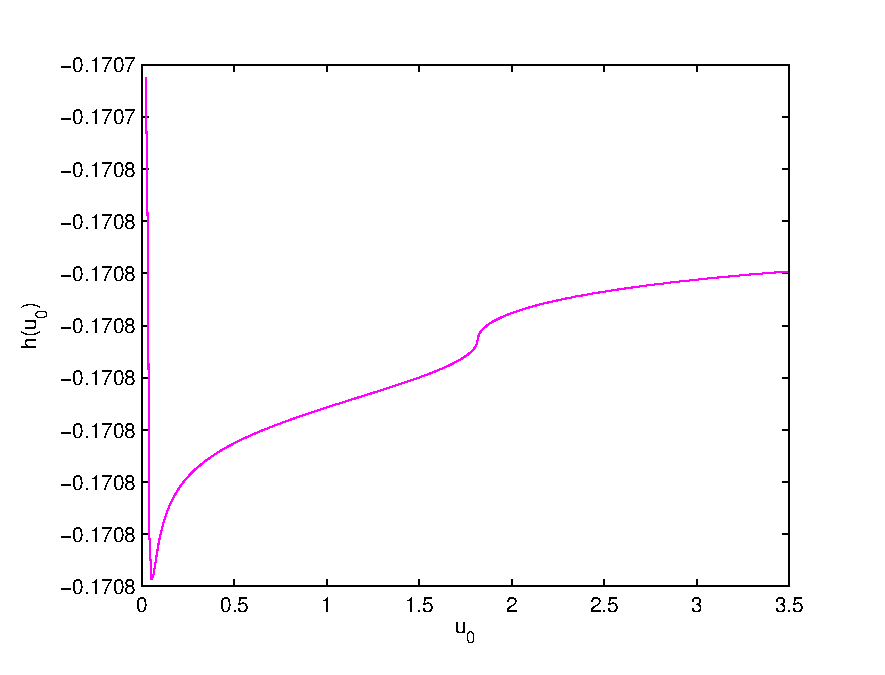
\includegraphics[scale=1.0]{pics/lyapunov_mid.eps}

\includegraphics[scale=1.0]{pics/lyapunov_small.eps}

Графики явно подтверждают, что хаотическое поведение в данной системе, описывающей популяцию одного из видов планктона, отсутствует. Показатель Ляпунова для любой начальной точки отрицателен, а значит, система обладает единственным устойчивым положением равновесия, являющимся глобальным аттрактором системы.
\pagebreak
\section{Исследование двумерной системы}
Рассмотрим следующую двумерную систему:
$$
n_{t+1} = n_t \exp{ \left\{ \frac{0.081}{n_t} - \frac{0.001}{n_{t-1}^2} - 0.305 \right\} }.
$$
Перепишем её в виде системы без запаздывания, введя новые переменные:
$$
\left\{
\begin{aligned}
u_{t+1} = u_t \exp{ \left\{ \frac{0.081}{u_t} - \frac{0.001}{v_t^2} - 0.305 \right\} }, \\
v_{t+1} = u_t.
\end{aligned}
\right.
$$
Для краткости будем записывать правую часть системы как $F(X) = [F_1(X), F_2(X)]^T$, где $X = [u, v]^T \in \mathbb{R}^2$. Компоненты неподвижных точек этой системы сопадают с неподвижными точками ранее исследованной одномерной системы, так как являются решениями одного и того же уравнения:
\begin{gather}
\left\{ \begin{aligned}
u_{t+1} = u_t, \\
v_{t+1} = v_t
\end{aligned} \right. \notag \\
\exp{ \left\{ \frac{0.081}{u_t} - \frac{0.001}{v_t^2} - 0.305 \right\} } = 1, \notag \\
\left\{ \begin{aligned}
\frac{0.081}{u_t} - \frac{0.001}{v_t^2} - 0.305 = 0, \\
v_{t+1} = u_t = v_t = u_{t-1}
\end{aligned} \right. \notag \\
\Rightarrow \frac{0.081}{u} - \frac{0.001}{u^2} - 0.305 = 0 \; \; \; (u_t = u). \notag
\end{gather}
\begin{theorem}
Пусть у дискретной динамической системы $X_{t+1} = F(X_t), X_t \in  \mathbb{R}^n$, правая часть есть гладкая функция. Тогда, если $X^*$ --- неподвижная точка этой системы, то ограниченность единицей модулей всех собственных значений якобиана, взятого в $X^*$ влечёт ассимптотическую устойчивость $X^*$. Если хоть одно собственное значение по модулю больше единицы, то $X^*$ неустойчива.
\end{theorem}

В нашем случае якобиан имеет вид:
\begin{gather}
J(u, v) = \left[ \begin{array}{ccc}
\frac{\partial F_1}{\partial u} & \frac{\partial F_1}{\partial v} \\[0.5em]
\frac{\partial F_2}{\partial u} & \frac{\partial F_2}{\partial v}
\end{array} \right] = \notag \\
= \left[ \begin{array}{ccc}
\exp{ \left\{ \frac{0.081}{u} - \frac{0.001}{v^2} - 0.305 \right\} }\left( 1 - \frac{0.081}{u} \right) &  0.002 \frac{u}{v^3} \exp{ \left\{ \frac{0.081}{u} - \frac{0.001}{v^2} - 0.305 \right\} } \\[0.5em]
1 & 0
\end{array} \right] \notag
\end{gather}

В неподвижной точке $(u_1^*, u_1^*)$ якобиан равен:
$$
J(u_1^*, u_1^*) \approx \left[ \begin{array}{ccc}
-5.240326895276133 & 11.870653790552266 \\[0.5em]
1 & 0
\end{array} \right],
$$
а его собственные числа $\lambda_1 \approx 1.708336325134350$, $\lambda_2 \approx -6.948663220410483$. Значит, точка $(u_1^*, u_1^*)$ --- неустойчивая неподвижная точка отображения.

В неподвижной точке $(u_2^*, u_2^*)$ якобиан равен:
$$
J(u_2^*, u_2^*) \approx \left[ \begin{array}{ccc}
0.679326895276141 & 0.031346209447718 \\[0.5em]
1 & 0
\end{array} \right],
$$
а его собственные числа $\lambda_1 \approx 0.722700609163030$, $\lambda_2 \approx -0.043373713886889$. Значит, точка $(u_2^*, u_2^*)$ --- устойчивая неподвижная точка отображения.

Рассмотрим двумерную динамическую систему с дискретным временем:
$$
u \rightarrow f(u, r), \; \; \; u \in \mathbb{R}^2, \; r \in \mathbb{R}
$$
\begin{definition}
Бифуркация положения равновесия в системе, соответствующая появлению собственных значений якобиана $\abs{\lambda_1} = \abs{\lambda_2} = 1, \lambda_1 = \overline{\lambda_2}, \lambda_1 \neq \lambda_2$, называется бифуркацией Неймарка--Сакера или дискретной бифуркацией Хопфа.
\end{definition}

Данная система не обладает бифуркациями типа Неймарка--Сакера, так как все собственные значения во всех положениях равновесия вещественны.

Примеры фазовых портретов системы (красными кругами обозначены неподвижные точки):

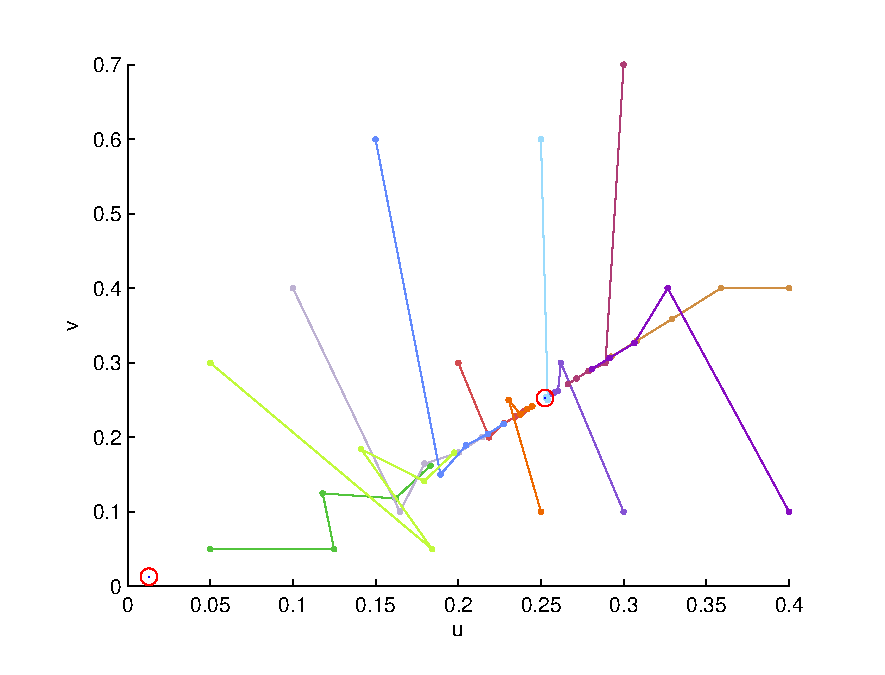
\includegraphics[scale=1.0]{pics/2dim_system.eps}

\pagebreak
\addcontentsline{toc}{section}{Список литературы}
\begin{thebibliography}{99}
\bibitem{Bratus} Братусь~А.~С., Новожилов~А.~С., Платонов~А.~П. Динамические системы и модели биологии. М.:~Физмалит, 2010.
\bibitem{Sharkovsky} Шарковский~А.~Н. Существование циклов непрерывного преобразования прямой в себя. Укр.~мат.~журн., т.~16, 1964. Стр. 61-65.
\end{thebibliography}
\end{document}
